% =====================================================================
%  Caminho de dados Uniciclo RISC-V32I -- conforme implementado em riscv_cpu.v
%  Versao STANDALONE (preview).  Compile:  pdflatex datapath_uniciclo.tex
% =====================================================================
\documentclass[border=10pt]{standalone}
\usepackage[T1]{fontenc}
\usepackage[utf8]{inputenc}
\usepackage{tikz}
\usetikzlibrary{positioning,calc,arrows.meta,backgrounds}

\tikzset{
  blk/.style ={draw,rounded corners=2pt,fill=blue!5,align=center,font=\small,line width=.5pt},
  mem/.style ={draw,fill=orange!12,align=center,font=\small,line width=.5pt},
  ctl/.style ={draw,rounded corners=6pt,fill=green!8,align=center,font=\footnotesize,line width=.5pt},
  wire/.style={-{Latex[length=2mm]},line width=.5pt},
  bus/.style ={-{Latex[length=2mm]},line width=1pt},
  ctrl/.style={-{Latex[length=1.6mm]},densely dashed,red!75!black,line width=.6pt},
  lbl/.style ={font=\scriptsize,inner sep=1pt},
  clbl/.style={font=\scriptsize,inner sep=1pt,text=red!75!black},
}

% mux 2:1 (trapezio): #1 id  #2 x  #3 y
\newcommand{\muxx}[3]{%
  \draw[fill=black!8,line width=.5pt]
    (#2-0.26,#3+0.62) -- (#2+0.26,#3+0.34) -- (#2+0.26,#3-0.34) -- (#2-0.26,#3-0.62) -- cycle;
  \coordinate (#1i0)  at (#2-0.26,#3+0.40);
  \coordinate (#1i1)  at (#2-0.26,#3-0.40);
  \coordinate (#1o)   at (#2+0.26,#3);
  \coordinate (#1sel) at (#2,#3-0.48);
  \node[lbl] at (#2-0.12,#3+0.40){0};
  \node[lbl] at (#2-0.12,#3-0.40){1};
}
% somador: #1 id  #2 x  #3 y
\newcommand{\adderx}[3]{%
  \draw[fill=blue!6,line width=.5pt] (#2,#3) circle(0.42);
  \node at (#2,#3){$+$};
  \coordinate (#1a) at (#2-0.40,#3+0.17);
  \coordinate (#1b) at (#2-0.40,#3-0.17);
  \coordinate (#1o) at (#2+0.42,#3);
}
% ULA (seta entalhada): #1 id  #2 x  #3 y
\newcommand{\aluu}[3]{%
  \draw[fill=blue!6,line width=.5pt]
    (#2-0.85,#3+0.95) -- (#2+0.85,#3+0.45) -- (#2+0.85,#3-0.45) -- (#2-0.85,#3-0.95)
    -- (#2-0.85,#3-0.32) -- (#2-0.45,#3) -- (#2-0.85,#3+0.32) -- cycle;
  \node[font=\small] at (#2+0.02,#3){ULA};
  \coordinate (#1a) at (#2-0.85,#3+0.58);
  \coordinate (#1b) at (#2-0.85,#3-0.58);
  \coordinate (#1o) at (#2+0.85,#3-0.18);
  \coordinate (#1z) at (#2+0.85,#3+0.05);
}

\begin{document}
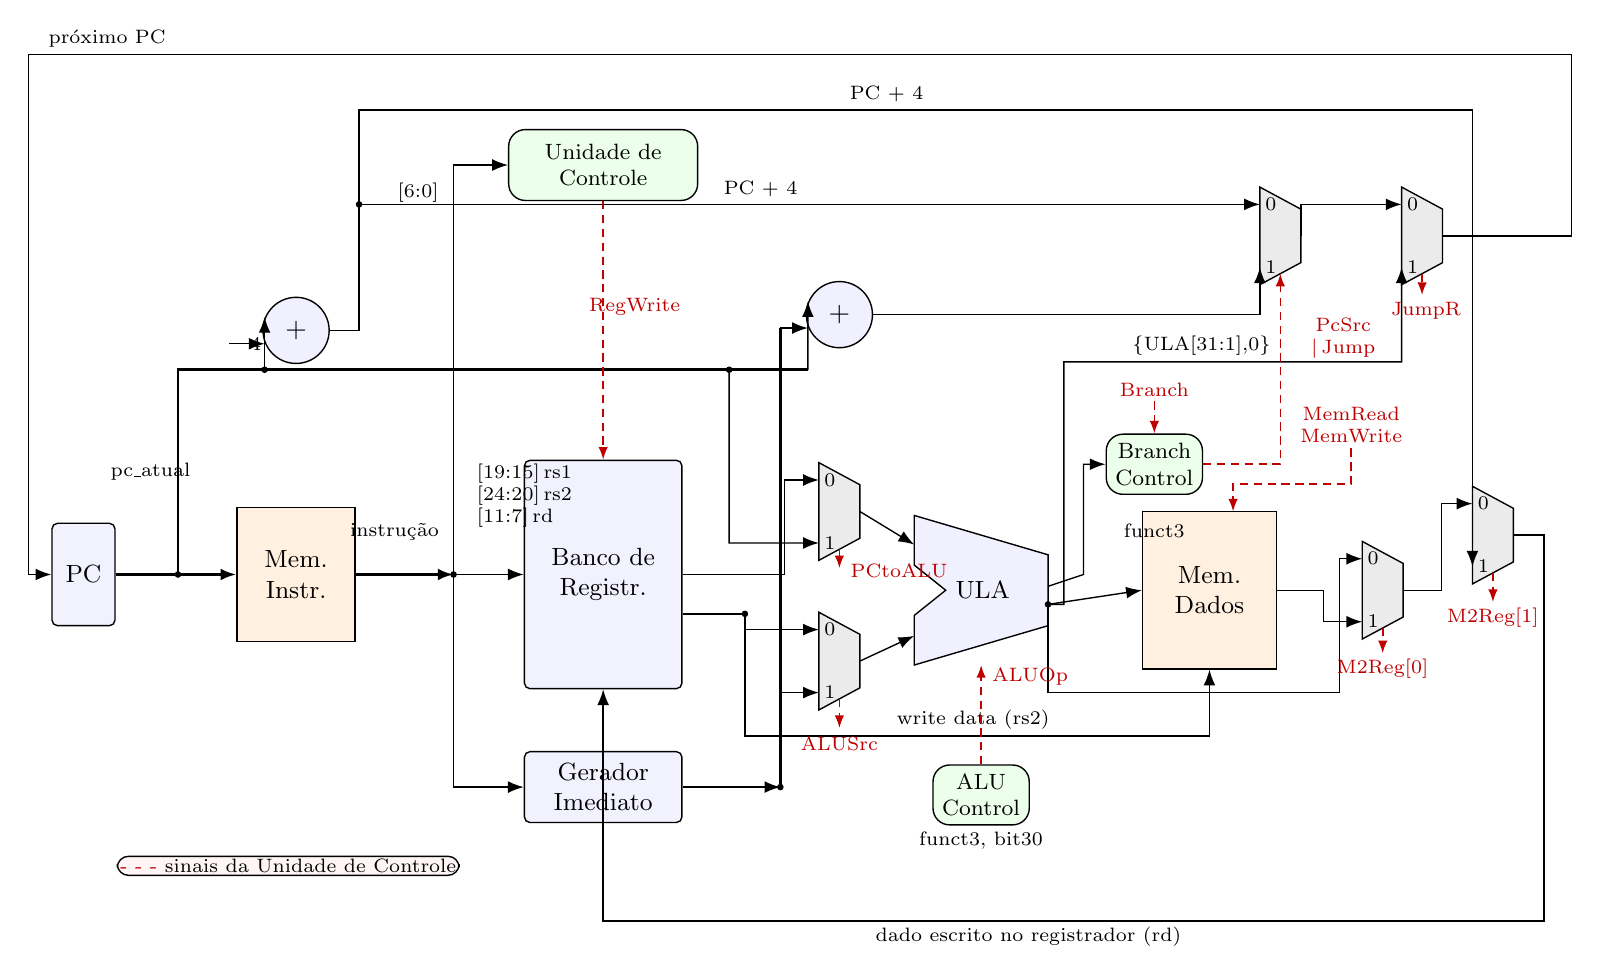
\begin{tikzpicture}[line width=.5pt]

% ===================== BLOCOS =======================================
\node[blk,minimum width=0.8cm,minimum height=1.3cm] (pc)  at (0,0)      {PC};
\node[mem,minimum width=1.5cm,minimum height=1.7cm] (im)  at (2.7,0)    {Mem.\\Instr.};
\node[blk,minimum width=2.0cm,minimum height=2.9cm] (reg) at (6.6,0)    {Banco de\\Registr.};
\node[blk,minimum width=2.0cm,minimum height=0.9cm] (imm) at (6.6,-2.7) {Gerador\\Imediato};
\aluu{alu}{11.4}{-0.2}
\node[mem,minimum width=1.7cm,minimum height=2.0cm] (dm)  at (14.3,-0.2){Mem.\\Dados};

\muxx{mxa}{9.6}{0.8}     % PCtoALU -> operando A
\muxx{mxb}{9.6}{-1.1}    % ALUSrc  -> operando B
\muxx{mw0}{16.5}{-0.2}   % MemtoReg[0]
\muxx{mw1}{17.9}{0.5}    % MemtoReg[1]

\adderx{a4}{2.7}{3.1}    % PC+4
\adderx{abr}{9.6}{3.3}   % PC+imediato
\muxx{mp0}{15.2}{4.3}    % PcSrc|Jump
\muxx{mp1}{17.0}{4.3}    % JumpR

\node[ctl,minimum width=2.4cm,minimum height=0.9cm] (cu) at (6.6,5.2){Unidade de\\Controle};
\node[ctl] (bc) at (13.6,1.4){Branch\\Control};
\node[ctl] (ac) at (11.4,-2.8){ALU\\Control};

% ===================== BUSCA ========================================
\draw[bus] (pc.east) -- (im.west);
\draw[line width=1pt] (1.2,0) -- (1.2,2.6) -- (9.2,2.6);
\fill (1.2,0) circle(1.2pt);
\draw[wire] (2.3,2.6) -- (a4a);
\draw[wire] (9.2,2.6) -- (abra);
\draw[wire] (8.2,2.6) -- (8.2,0.4) -- (mxai1);
\fill (8.2,2.6) circle(1.2pt); \fill (2.3,2.6) circle(1.2pt);
\node[lbl] at (0.85,1.3){pc\_atual};
\node[lbl,left=0pt of a4b]{4};
\draw[wire] ($(a4b)+(-0.45,0)$) -- (a4b);

\draw[bus] (im.east) -- (4.7,0);
\fill (4.7,0) circle(1.2pt);
\node[lbl] at (3.95,0.55){instru\c{c}\~ao};
\draw[wire] (4.7,0) -- (reg.west);
\node[lbl,align=left] at (5.6,1.0){[19:15]\,rs1\\ {[24:20]}\,rs2\\ {[11:7]}\,rd};
\draw[wire] (4.7,0) |- (imm.west);
\draw[wire] (4.7,0) -- (4.7,5.2) -- (cu.west);
\node[lbl] at (4.25,4.85){[6:0]};

% ===================== REG / IMM / ULA ==============================
\draw[wire] (reg.east) -- (8.9,0.0) |- (mxai0);
\draw[wire] ($(reg.east)+(0,-0.5)$) -- (8.4,-0.5) |- (mxbi0);
\fill (8.4,-0.5) circle(1.2pt);
\draw[wire] (8.4,-0.5) -- (8.4,-2.05) -- (14.3,-2.05) -- (dm.south);
\node[lbl] at (11.3,-1.85){write data (rs2)};

\draw[wire] (imm.east) -- (8.85,-2.7);
\fill (8.85,-2.7) circle(1.2pt);
\draw[wire] (8.85,-2.7) |- (mxbi1);
\draw[line width=1pt] (8.85,-2.7) -- (8.85,3.13);
\draw[wire] (8.85,3.13) -- (abrb);

\draw[wire] (mxao) -- (alua);
\draw[wire] (mxbo) -- (alub);

% ===================== ULA -> MEM / WB ==============================
\draw[wire] (aluo) -- (dm.west);
\fill (aluo) circle(1.2pt);
\draw[wire] (aluo) -- (12.25,-1.5) -- (15.95,-1.5) -- (15.95,0.2) -- (mw0i0); % resultado -> WB0 in0
\draw[wire] (aluz) -- (12.7,0.0) -- (12.7,1.4) -- (bc.west);                  % zero -> branch ctrl
\draw[wire] (dm.east) -- (15.75,-0.2) |- (mw0i1);
\draw[wire] (mw0o) -- (17.25,-0.2) |- (mw1i0);
\draw[wire] (mw1o) -- (18.55,0.5) -- (18.55,-4.4) -- (6.6,-4.4) -- (reg.south);
\node[lbl] at (12.0,-4.6){dado escrito no registrador (rd)};

% ===================== PROXIMO PC ===================================
\draw[wire] (a4o) -- (3.5,3.1) -- (3.5,4.7) -- (mp0i0);
\fill (3.5,4.7) circle(1.2pt);
\draw[wire] (3.5,4.7) -- (3.5,5.9) -- (17.64,5.9) -- (mw1i1);     % PC+4 -> WB1 in1
\node[lbl] at (10.2,6.1){PC + 4};
\node[lbl] at (8.6,4.9){PC + 4};

\draw[wire] (abro) -| (mp0i1);                                   % PC+imm -> mux in1
\draw[wire] (mp0o) |- (mp1i0);                                   % -> mp1 in0
\draw[wire] (aluo) -- (12.45,-0.38) -- (12.45,2.7) -- (16.74,2.7) -- (mp1i1); % jalr alvo
\node[lbl,align=center] at (14.2,2.9){\{ULA[31:1],0\}};
\draw[wire] (mp1o) -- (18.9,4.3) -- (18.9,6.6) -- (-0.7,6.6) -- (-0.7,0) -- (pc.west);
\node[lbl] at (0.3,6.8){pr\'oximo PC};

% ===================== CONTROLE (tracejado) =========================
\draw[ctrl] (cu.south) -- (reg.north);
\node[clbl] at (7.0,3.4){RegWrite};
\draw[ctrl] (mxbsel) -- (9.6,-1.95);  \node[clbl] at (9.6,-2.15){ALUSrc};
\draw[ctrl] (mxasel) -- (9.6,0.08);   \node[clbl,right] at (9.7,0.05){PCtoALU};
\draw[ctrl] (mw0sel) -- (16.5,-1.0);  \node[clbl] at (16.5,-1.2){M2Reg[0]};
\draw[ctrl] (mw1sel) -- (17.9,-0.35); \node[clbl] at (17.9,-0.55){M2Reg[1]};
\draw[ctrl] (bc.east) -- (15.2,1.4) -- (mp0sel);  \node[clbl,align=center] at (16.0,3.0){PcSrc\\$|$\,Jump};
\draw[ctrl] (mp1sel) -- (17.0,3.55);  \node[clbl] at (17.05,3.35){JumpR};
\draw[ctrl] (ac.north) -- (11.4,-1.15); \node[clbl,right] at (11.5,-1.3){ALUOp};
% sinais que chegam dos blocos de controle (stubs)
\draw[ctrl] (13.6,2.2) -- (bc.north); \node[clbl] at (13.6,2.35){Branch};
\draw[ctrl] (16.1,1.6) -- (16.1,1.15) -- (14.6,1.15) -- (14.6,0.8); \node[clbl,align=center] at (16.1,1.9){MemRead\\MemWrite};
\node[lbl,below=1pt of ac]{funct3, bit30};
\node[lbl] at (13.6,0.55){funct3};

\node[lbl,draw,rounded corners,fill=red!4] at (2.6,-3.7)
  {\textcolor{red!75!black}{- - -} sinais da Unidade de Controle};

\end{tikzpicture}
\end{document}
